\hypertarget{thingsboard}{%
\chapter{ThingsBoard}\label{thingsboard}}

\section*{Objetivos de Aprendizagem}

Ao final deste capítulo, o leitor será capaz de:

\begin{itemize}
\tightlist
\item
  Explicar o papel do ThingsBoard em uma arquitetura de supervisão e onde ele \textbf{não} deve ser usado.
\item
  Descrever o modelo de entidades da plataforma: locatário, cliente, dispositivo, ativo e perfil.
\item
  Distinguir telemetria de atributos e os escopos de atributo.
\item
  Publicar telemetria por MQTT e por HTTP e explicar o formato do \emph{payload}.
\item
  Construir uma \emph{rule chain} que persiste telemetria e cria e limpa um alarme.
\item
  Distinguir RPC do lado do servidor e do lado do dispositivo.
\item
  Integrar CLP e Node-RED a uma instância ThingsBoard, inclusive por \emph{gateway}.
\item
  Montar um dashboard com telemetria, atributos e alarmes.
\end{itemize}

\begin{center}\rule{0.5\linewidth}{0.5pt}\end{center}

\hypertarget{o-que-uxe9-o-thingsboard-e-onde-ele-se-encaixa}{%
\section{O que é o ThingsBoard e onde ele se encaixa}\label{o-que-uxe9-o-thingsboard-e-onde-ele-se-encaixa}}

O ThingsBoard é uma plataforma de código aberto para \textbf{coleta, processamento, visualização e gestão de dados de dispositivos IoT e IIoT}. Ele oferece três modos de uso:

\textbf{Tabela 12.1 -- Modos de uso}

\begin{longtable}[]{@{}
  >{\raggedright\arraybackslash}p{(\columnwidth - 4\tabcolsep) * \real{0.3333}}
  >{\raggedright\arraybackslash}p{(\columnwidth - 4\tabcolsep) * \real{0.3333}}
  >{\raggedright\arraybackslash}p{(\columnwidth - 4\tabcolsep) * \real{0.3333}}@{}}
\toprule\noalign{}
\begin{minipage}[b]{\linewidth}\raggedright
Modo
\end{minipage} & \begin{minipage}[b]{\linewidth}\raggedright
O que é
\end{minipage} & \begin{minipage}[b]{\linewidth}\raggedright
Quando faz sentido
\end{minipage} \\
\midrule\noalign{}
\endhead
\bottomrule\noalign{}
\endlastfoot
Community Edition (CE) & Código aberto, instalado pelo usuário & Estudo, laboratório, piloto, projeto com controle total da infraestrutura \\
Professional Edition (PE) & Distribuição com recursos adicionais de gestão e integração & Operação comercial com requisitos de suporte e escala \\
ThingsBoard Cloud & Serviço gerenciado & Prova de conceito rápida, sem infraestrutura própria \\
\end{longtable}

A documentação oficial concentra a maior parte dos exemplos em três domínios equivalentes: o \emph{site} principal (\passthrough{\lstinline!thingsboard.io/docs!}), a versão profissional (\passthrough{\lstinline!/docs/pe/!}) e a nuvem (\passthrough{\lstinline!/docs/paas/!}). A API de dispositivo, no entanto, é a mesma --- o que aprende no laboratório vale na operação.

\textbf{Onde ele se encaixa.} O ThingsBoard entra na camada de \textbf{integração, telemetria, alarme informativo e visualização} de frotas de dispositivos. Ele não substitui o CLP (controle e proteção) nem o SCADA (operação e comando do processo em tempo real).

\begin{center}
\IfFileExists{../figuras/capitulo-12-m1.pdf}{%
  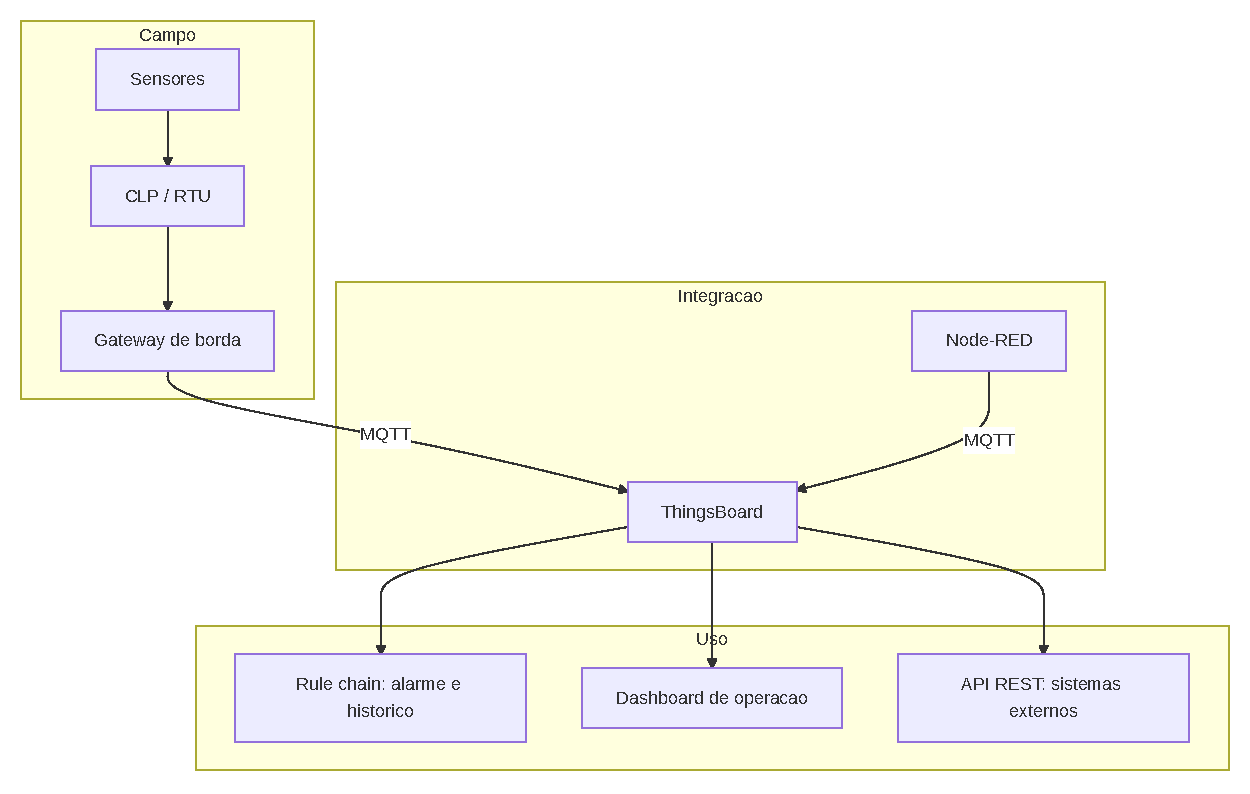
\includegraphics[width=\linewidth,height=0.8\textheight,keepaspectratio]{../figuras/capitulo-12-m1.pdf}%
}{\fbox{\parbox{0.9\linewidth}{\small Diagrama Mermaid ainda não renderizado: capitulo-12-m1. Rode scripts/render-mermaid.sh.}}}
\end{center}

\begin{caixaatencao}

\textbf{Atenção:} o ThingsBoard \textbf{não} é sistema de comando de processo. Comandos enviados por \emph{dashboards} em nuvem dependem de rede, proxy e disponibilidade da plataforma --- nenhum deles é adequado a uma função de segurança ou de controle em malha fechada. Use a plataforma para supervisão, diagnóstico, manutenção e análise; mantenha proteção e controle no CLP.

\end{caixaatencao}

\begin{center}\rule{0.5\linewidth}{0.5pt}\end{center}

\hypertarget{modelo-de-entidades}{%
\section{Modelo de entidades}\label{modelo-de-entidades}}

Entender o modelo de entidades é o que separa ``usar a plataforma'' de ``usar a plataforma corretamente''.

\textbf{Tabela 12.2 -- Entidades principais}

\begin{longtable}[]{@{}
  >{\raggedright\arraybackslash}p{(\columnwidth - 4\tabcolsep) * \real{0.3333}}
  >{\raggedright\arraybackslash}p{(\columnwidth - 4\tabcolsep) * \real{0.3333}}
  >{\raggedright\arraybackslash}p{(\columnwidth - 4\tabcolsep) * \real{0.3333}}@{}}
\toprule\noalign{}
\begin{minipage}[b]{\linewidth}\raggedright
Entidade
\end{minipage} & \begin{minipage}[b]{\linewidth}\raggedright
Papel
\end{minipage} & \begin{minipage}[b]{\linewidth}\raggedright
Exemplo na planta
\end{minipage} \\
\midrule\noalign{}
\endhead
\bottomrule\noalign{}
\endlastfoot
\textbf{Locatário} (\emph{tenant}) & Instância do cliente, raiz dos dados & A concessionária \\
\textbf{Cliente} (\emph{customer}) & Subdivisão de negócio dentro do locatário & Município atendido \\
\textbf{Dispositivo} (\emph{device}) & Ativo que publica dados & Gateway da estação, transmissor \\
\textbf{Ativo} (\emph{asset}) & Agrupamento lógico de dispositivos & Estação elevatória 1, adutora norte \\
\textbf{Perfil de dispositivo} (\emph{device profile}) & Modelo com comportamento comum & Perfil ``transmissor de pressão'' \\
\textbf{Grupo de entidades} (\emph{entity group}) & Agrupamento para permissões e consultas & Bombas críticas \\
\end{longtable}

A hierarquia recomendada para processo industrial é: \textbf{ativo} representa a instalação física (estação, subestação, adutora) e \textbf{dispositivo} representa o equipamento conectado. Relações explícitas entre ativos e dispositivos permitem consultar ``todas as variáveis da estação 1'' sem armazenar isso no nome de cada dispositivo.

\begin{caixadica}

\textbf{Dica:} nomes de entidade são interface. \passthrough{\lstinline!EST1-BOMBA2-TEMP-MANCAL!} informa; \passthrough{\lstinline!device\_0017!} não. Em projeto com mais de vinte dispositivos, um padrão de nomenclatura definido antes do cadastro vale mais que qualquer recurso da plataforma.

\end{caixadica}

\begin{center}\rule{0.5\linewidth}{0.5pt}\end{center}

\hypertarget{telemetria-e-atributos}{%
\section{Telemetria e atributos}\label{telemetria-e-atributos}}

A distinção é conceitual e tem consequência direta em custo de armazenamento e desempenho.

\textbf{Tabela 12.3 -- Telemetria \ensuremath{\times} atributos}

\begin{longtable}[]{@{}
  >{\raggedright\arraybackslash}p{(\columnwidth - 4\tabcolsep) * \real{0.3333}}
  >{\raggedright\arraybackslash}p{(\columnwidth - 4\tabcolsep) * \real{0.3333}}
  >{\raggedright\arraybackslash}p{(\columnwidth - 4\tabcolsep) * \real{0.3333}}@{}}
\toprule\noalign{}
\begin{minipage}[b]{\linewidth}\raggedright
Aspecto
\end{minipage} & \begin{minipage}[b]{\linewidth}\raggedright
Telemetria
\end{minipage} & \begin{minipage}[b]{\linewidth}\raggedright
Atributos
\end{minipage} \\
\midrule\noalign{}
\endhead
\bottomrule\noalign{}
\endlastfoot
Natureza & Série temporal: cada valor é um ponto no tempo & Valor de estado: o último valor substitui o anterior \\
Exemplo & Temperatura, pressão, vazão & Número de série, versão de firmware, faixa de medição \\
Armazenamento & Histórico com todos os pontos & Apenas valor atual por chave \\
Escopo & Único & Cliente, compartilhado e servidor \\
\end{longtable}

Os \textbf{escopos de atributo} definem quem lê e quem escreve:

\begin{itemize}
\tightlist
\item
  \textbf{Atributo de servidor} (\emph{server scope}): gerenciado apenas pela plataforma e pela API; o dispositivo não vê. Útil para dados de gestão, contrato e configuração central.
\item
  \textbf{Atributo compartilhado} (\emph{shared scope}): definido na plataforma e \textbf{enviado ao dispositivo}. É o mecanismo de configuração remota, como intervalo de amostragem ou limite de alarme.
\item
  \textbf{Atributo de cliente} (\emph{client scope}): publicado pelo dispositivo e visível na plataforma. Útil para metadados do próprio equipamento.
\end{itemize}

\hypertarget{mqtt-tuxf3picos-e-formato}{%
\subsection{MQTT: tópicos e formato}\label{mqtt-tuxf3picos-e-formato}}

O dispositivo autentica com o \textbf{token de acesso} e publica em tópicos definidos.

\textbf{Tabela 12.4 -- Tópicos MQTT de dispositivo}

\begin{longtable}[]{@{}
  >{\raggedright\arraybackslash}p{(\columnwidth - 4\tabcolsep) * \real{0.3333}}
  >{\raggedright\arraybackslash}p{(\columnwidth - 4\tabcolsep) * \real{0.3333}}
  >{\raggedright\arraybackslash}p{(\columnwidth - 4\tabcolsep) * \real{0.3333}}@{}}
\toprule\noalign{}
\begin{minipage}[b]{\linewidth}\raggedright
Operação
\end{minipage} & \begin{minipage}[b]{\linewidth}\raggedright
Tópico padrão
\end{minipage} & \begin{minipage}[b]{\linewidth}\raggedright
Forma curta
\end{minipage} \\
\midrule\noalign{}
\endhead
\bottomrule\noalign{}
\endlastfoot
Publicar telemetria & \passthrough{\lstinline!v1/devices/me/telemetry!} & \passthrough{\lstinline!v2/t!} \\
Publicar atributo de cliente & \passthrough{\lstinline!v1/devices/me/attributes!} & --- \\
Assinar atributo compartilhado & \passthrough{\lstinline!v1/devices/me/attributes!} & --- \\
Assinar RPC do servidor & \passthrough{\lstinline!v1/devices/me/rpc/request/+!} & --- \\
Requisição RPC do dispositivo & \passthrough{\lstinline!v1/devices/me/rpc/request/$id!} & \passthrough{\lstinline!v2/r/req/$id!} \\
Resposta de RPC do dispositivo & \passthrough{\lstinline!v1/devices/me/rpc/response/$id!} & \passthrough{\lstinline!v2/r/res/+!} \\
\end{longtable}

Formatos de \emph{payload} aceitos para telemetria:

\begin{lstlisting}
{"temperature": 22.5, "humidity": 61}
\end{lstlisting}

\begin{lstlisting}
{"ts": 1757429087063, "values": {"temperature": 22.5}}
\end{lstlisting}

\begin{lstlisting}
[
  {"ts": 1757429080000, "values": {"temperature": 22.5}},
  {"ts": 1757429090000, "values": {"temperature": 22.7}}
]
\end{lstlisting}

O primeiro formato usa o horário de recebimento na plataforma. O segundo e o terceiro usam \textbf{timestamp do dispositivo} (\passthrough{\lstinline!ts!}, em milissegundos Unix) --- indispensável quando a publicação pode atrasar, como em enlace de rádio ou \emph{store and forward} na borda.

\begin{caixaatencao}

\textbf{Atenção:} sem \emph{timestamp} do dispositivo, todo dado que chega atrasado é gravado com a hora de chegada. Em enlace instável isso produz séries temporais que mentem: uma leitura de duas horas atrás aparece como atual. Se o seu \emph{gateway} tem fila local, \textbf{sempre} envie \passthrough{\lstinline!ts!}.

\end{caixaatencao}

\hypertarget{http-e-rest}{%
\subsection{HTTP e REST}\label{http-e-rest}}

Para dispositivos sem MQTT ou para integração com sistemas externos, a plataforma expõe:

\begin{lstlisting}
POST https://<host>/api/v1/$ACCESS_TOKEN/telemetry
POST /api/plugins/telemetry/{tipoEntidade}/{id}/attributes/{escopo}
\end{lstlisting}

A mesma estrutura de \emph{payload} é aceita. O segundo \emph{endpoint} é usado por aplicações com credencial de usuário (API REST administrativa), não pelo dispositivo.

\begin{center}\rule{0.5\linewidth}{0.5pt}\end{center}

\hypertarget{rule-engine}{%
\section{Rule engine}\label{rule-engine}}

O motor de regras é o núcleo de processamento: cada mensagem (telemetria, alteração de atributo, evento de ciclo de vida, chamada RPC) percorre uma \textbf{rule chain} (\emph{cadeia de regras}), composta por nós conectados.

\begin{center}
\IfFileExists{../figuras/capitulo-12-m2.pdf}{%
  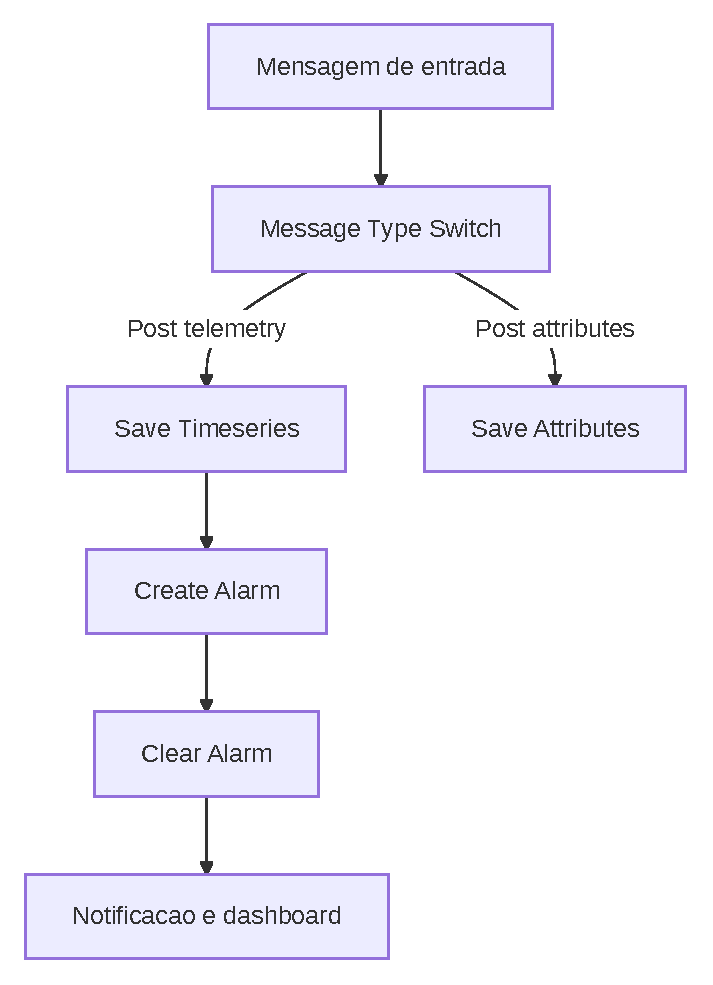
\includegraphics[width=\linewidth,height=0.8\textheight,keepaspectratio]{../figuras/capitulo-12-m2.pdf}%
}{\fbox{\parbox{0.9\linewidth}{\small Diagrama Mermaid ainda não renderizado: capitulo-12-m2. Rode scripts/render-mermaid.sh.}}}
\end{center}

Nós mais usados em um projeto de supervisão:

\begin{longtable}[]{@{}
  >{\raggedright\arraybackslash}p{(\columnwidth - 2\tabcolsep) * \real{0.5000}}
  >{\raggedright\arraybackslash}p{(\columnwidth - 2\tabcolsep) * \real{0.5000}}@{}}
\toprule\noalign{}
\begin{minipage}[b]{\linewidth}\raggedright
Nó
\end{minipage} & \begin{minipage}[b]{\linewidth}\raggedright
Função
\end{minipage} \\
\midrule\noalign{}
\endhead
\bottomrule\noalign{}
\endlastfoot
Message Type Switch & Encaminha conforme o tipo da mensagem (telemetria, atributo, RPC) \\
Save Timeseries & Persiste a telemetria com retenção configurável \\
Save Attributes & Grava atributos no escopo definido \\
Create Alarm & Cria ou atualiza um alarme a partir da condição avaliada \\
Clear Alarm & Encerra o alarme quando a condição cessa \\
Fetch Device Info & Enriquece a mensagem com dados da entidade de origem \\
Kafka / MQTT / REST & Publica a mensagem em sistemas externos \\
\end{longtable}

\begin{caixafigura}

\textbf{{[}Figura 12.1 -- Editor de rule chain com o fluxo de alarme{]}}
\emph{Captura do editor com quatro nós conectados: Message Type Switch, Save Timeseries, Create Alarm e Clear Alarm. Anotar as saídas ``Post telemetry'', ``Success'' e ``Alarm created''; destacar onde ficam o tipo do alarme e a severidade. Interface em inglês, captura genérica.}

\end{caixafigura}

Um nó comum é o \textbf{Message Type Switch}, que separa o fluxo: mensagens \passthrough{\lstinline!Post telemetry!}, \passthrough{\lstinline!Post attributes!} e \passthrough{\lstinline!RPC Request!} seguem caminhos diferentes na mesma cadeia.

\hypertarget{alarme-como-entidade}{%
\subsection{Alarme como entidade}\label{alarme-como-entidade}}

No ThingsBoard o alarme é uma \textbf{entidade} com estado. Os campos relevantes observáveis na documentação oficial:

\begin{itemize}
\tightlist
\item
  \textbf{Tipo} (\emph{type}), como \passthrough{\lstinline!High Temperature!}.
\item
  \textbf{Severidade} (\emph{severity}): \passthrough{\lstinline!CRITICAL!}, \passthrough{\lstinline!MAJOR!}, \passthrough{\lstinline!MINOR!}, \passthrough{\lstinline!WARNING!}, \passthrough{\lstinline!INDETERMINATE!}.
\item
  \textbf{Origem} (\emph{originator}): dispositivo ou ativo que gerou.
\item
  \textbf{Estado}: ativo não reconhecido (\passthrough{\lstinline!ACTIVE\_UNACK!}), ativo reconhecido, limpo não reconhecido, limpo reconhecido.
\item
  \textbf{Instantes} de início (\passthrough{\lstinline!startTs!}) e fim (\passthrough{\lstinline!endTs!}).
\item
  \textbf{Detalhes} (\emph{details}): valores do momento, definidos por script.
\end{itemize}

\begin{lstlisting}
{
  "scriptLang": "TBEL",
  "alarmType": "High Temperature",
  "severity": "CRITICAL",
  "alarmDetailsBuildTbel": "return { temperature: msg.temperature };"
}
\end{lstlisting}

O nó \textbf{Clear Alarm} encerra o alarme quando a condição normaliza --- e o \textbf{reconhecimento} é dado operacional, não de configuração: é o registro de que alguém assumiu o alarme.

\begin{caixanota}

\textbf{Atualização tecnológica:} o alarme em plataforma IIoT \textbf{não substitui} o gerenciamento de alarmes de processo do capítulo 10. Ele cobre o ciclo operacional de notificação, reconhecimento e histórico de uma frota de dispositivos, mas a filosofia de alarmes, a matriz de prioridade, a racionalização e o controle de mudanças continuam sendo o que dá qualidade ao sistema. Sem essas disciplinas, a plataforma apenas automatiza a produção de alarmes em excesso.

\end{caixanota}

\begin{center}\rule{0.5\linewidth}{0.5pt}\end{center}

\hypertarget{rpc-comando-e-consulta}{%
\section{\texorpdfstring{RPC --- comando e consulta}{RPC  comando e consulta}}\label{rpc-comando-e-consulta}}

RPC (\emph{Remote Procedure Call}) permite trocar comandos e respostas entre plataforma e dispositivo.

\begin{itemize}
\tightlist
\item
  \textbf{RPC do lado do servidor} (\emph{server-side}): a plataforma (ou um dashboard) envia um comando ao dispositivo. Exemplos: alterar intervalo de amostragem, solicitar leitura imediata, acionar reinício controlado.
\item
  \textbf{RPC do lado do dispositivo} (\emph{client-side}): o dispositivo solicita algo à plataforma por um tópico de requisição e recebe a resposta em outro.
\end{itemize}

\begin{lstlisting}
Dispositivo publica:  {"method": "getCurrentTime", "params": {}}
em v1/devices/me/rpc/request/42
Plataforma responde:  {"currentTime": 1757429087063}
em v1/devices/me/rpc/response/42
\end{lstlisting}

Cuidado de engenharia: RPC é um canal de \textbf{comando}, e comando exige autorização e auditoria. Antes de habilitar RPC de escrita em um dispositivo de processo, defina quem pode chamar, qual o efeito de um comando repetido (idempotência) e como o evento aparece no registro de auditoria.

\begin{center}\rule{0.5\linewidth}{0.5pt}\end{center}

\hypertarget{dashboards-e-visualizauxe7uxe3o}{%
\section{Dashboards e visualização}\label{dashboards-e-visualizauxe7uxe3o}}

Os dashboards da plataforma oferecem painéis de série temporal, indicadores, tabelas, mapas e widgets de alarme. O que muda em relação ao capítulo 11 é a \textbf{origem do dado}: aqui o painel consulta a própria plataforma, e não um banco externo.

Diretrizes que continuam valendo integralmente:

\begin{itemize}
\tightlist
\item
  Escala fixa em painéis de processo; unidade visível; precisão significativa.
\item
  Poucos indicadores por tela, com hierarquia clara.
\item
  Cor reservada para significado, não para estética.
\item
  Lista de alarmes separada do painel de indicadores --- no painel de operação, o alarme entra como destaque e como contagem por severidade.
\end{itemize}

\begin{caixafigura}

\textbf{{[}Figura 12.2 -- Dashboard de operação com telemetria, atributos e alarmes{]}}
\emph{Tela com quatro indicadores de processo com faixa normal, duas tendências (24 h), um widget de estado de alarme por severidade e uma tabela de dispositivos com último contato. Destacar o uso de escala fixa e a ausência de cor decorativa. Captura genérica, sem marca de terceiros.}

\end{caixafigura}

\begin{center}\rule{0.5\linewidth}{0.5pt}\end{center}

\hypertarget{integrauxe7uxe3o-com-clp-e-com-node-red}{%
\section{Integração com CLP e com Node-RED}\label{integrauxe7uxe3o-com-clp-e-com-node-red}}

\hypertarget{direto-do-clp}{%
\subsection{Direto do CLP}\label{direto-do-clp}}

CLPs com função de cliente MQTT publicam telemetria diretamente, desde que o \emph{payload} siga o formato esperado e o token esteja protegido. Como token em CLP é difícil de rotacionar, o padrão mais defensável é \textbf{não} expor a credencial no controlador.

\hypertarget{por-gateway-de-borda}{%
\subsection{Por gateway de borda}\label{por-gateway-de-borda}}

O \emph{gateway} concentra credenciais, fila local e conversão de protocolo. A plataforma define tópicos específicos para esse papel:

\textbf{Tabela 12.5 -- Tópicos MQTT de gateway (prefixo \passthrough{\lstinline!v1/gateway/!})}

\begin{longtable}[]{@{}
  >{\raggedright\arraybackslash}p{(\columnwidth - 4\tabcolsep) * \real{0.3333}}
  >{\raggedright\arraybackslash}p{(\columnwidth - 4\tabcolsep) * \real{0.3333}}
  >{\raggedright\arraybackslash}p{(\columnwidth - 4\tabcolsep) * \real{0.3333}}@{}}
\toprule\noalign{}
\begin{minipage}[b]{\linewidth}\raggedright
Tópico
\end{minipage} & \begin{minipage}[b]{\linewidth}\raggedright
Direção
\end{minipage} & \begin{minipage}[b]{\linewidth}\raggedright
Uso
\end{minipage} \\
\midrule\noalign{}
\endhead
\bottomrule\noalign{}
\endlastfoot
\passthrough{\lstinline!connect!} / \passthrough{\lstinline!disconnect!} & Publica & Anunciar conexão e desconexão de dispositivo subordinado \\
\passthrough{\lstinline!telemetry!} & Publica & Enviar telemetria de um ou vários dispositivos \\
\passthrough{\lstinline!attributes!} & Publica / Assina & Enviar atributos de cliente e receber atributos compartilhados \\
\passthrough{\lstinline!attributes/request!} e \passthrough{\lstinline!attributes/response!} & Publica / Assina & Solicitar valores de atributo \\
\passthrough{\lstinline!rpc!} & Assina / Publica & Receber comandos do servidor e enviar respostas \\
\passthrough{\lstinline!claim!} & Publica & Iniciar processo de reivindicação de dispositivo \\
\end{longtable}

Esse desenho é o que viabiliza o caso clássico: \textbf{um gateway para N dispositivos}, com uma única credencial e um único ponto de filtragem e buffer.

\begin{caixafigura}

\textbf{{[}Figura 12.3 -- Gateway de borda concentrando dispositivos para a plataforma{]}}
\emph{Diagrama com três CLPs e quatro transmissores de campo à esquerda; no centro, o gateway de borda com fila local e conversão de protocolo; à direita, a plataforma recebendo um único fluxo MQTT. Marcar com tracejado o caminho que permanece local quando o enlace cai. Sem logomarca de fabricante.}

\end{caixafigura}

\hypertarget{com-node-red}{%
\subsection{Com Node-RED}\label{com-node-red}}

O Node-RED atua como camada de integração e normalização --- papel discutido no capítulo 7:

\begin{lstlisting}
CLP -> Node-RED (Modbus TCP) -> normaliza -> MQTT -> ThingsBoard
\end{lstlisting}

Vantagens: conversão de unidades e escalas no fluxo, agregação, cálculo de indicadores antes da publicação (reduz volume na nuvem) e buffer em caso de queda de enlace.

\begin{caixaatencao}

\textbf{Atenção:} publique na nuvem a \textbf{taxa que a decisão exige}, não a taxa que o CLP produz. Publicar 50 variáveis a 100 ms gera gigabytes por mês de dado que ninguém vai analisar. Agregue na borda (média, máximo e mínimo por minuto) e mantenha a alta taxa apenas para diagnóstico sob demanda.

\end{caixaatencao}

\begin{center}\rule{0.5\linewidth}{0.5pt}\end{center}

\hypertarget{estudo-de-caso-monitoramento-de-frota-de-transmissores}{%
\section{\texorpdfstring{Estudo de caso --- monitoramento de frota de transmissores}{Estudo de caso  monitoramento de frota de transmissores}}\label{estudo-de-caso-monitoramento-de-frota-de-transmissores}}

\textbf{Cenário.} Uma estação de tratamento possui 24 transmissores de pressão e nível em campo, conectados a dois CLPs. Objetivo: acompanhar falhas de instrumento e condições anormais sem depender do operador para perceber o problema.

\textbf{Arquitetura.} CLP lê os transmissores; Node-RED na borda lê o CLP por Modbus TCP, normaliza escalas, calcula média de 1 minuto e publica em MQTT; um único \emph{gateway} ThingsBoard encaminha 24 dispositivos; a \emph{rule chain} persiste telemetria, cria alarme de desvio e de falha de comunicação e notifica a manutenção.

\textbf{Regras implementadas.}

\begin{longtable}[]{@{}
  >{\raggedright\arraybackslash}p{(\columnwidth - 4\tabcolsep) * \real{0.3333}}
  >{\raggedright\arraybackslash}p{(\columnwidth - 4\tabcolsep) * \real{0.3333}}
  >{\raggedright\arraybackslash}p{(\columnwidth - 4\tabcolsep) * \real{0.3333}}@{}}
\toprule\noalign{}
\begin{minipage}[b]{\linewidth}\raggedright
Condição
\end{minipage} & \begin{minipage}[b]{\linewidth}\raggedright
Alarme
\end{minipage} & \begin{minipage}[b]{\linewidth}\raggedright
Severidade
\end{minipage} \\
\midrule\noalign{}
\endhead
\bottomrule\noalign{}
\endlastfoot
Pressão fora da faixa por mais de 5 min & Desvio de processo & MAJOR \\
Valor com qualidade ruim por mais de 2 min & Falha de comunicação & CRITICAL \\
Sem mensagem por mais de 10 min & Dispositivo silencioso & CRITICAL \\
Bateria abaixo de 20\% (onde aplicável) & Manutenção preventiva & WARNING \\
\end{longtable}

\textbf{Decisões de projeto que fizeram diferença.}

\begin{enumerate}
\def\labelenumi{\arabic{enumi}.}
\tightlist
\item
  \textbf{Timestamp do dispositivo} mantido em todos os pontos, porque o enlace de rádio enfileira mensagens em dias de chuva.
\item
  \textbf{Alarme de comunicação separado} de alarme de processo --- o mesmo erro discutido no capítulo 10.
\item
  \textbf{Agregação na borda}: 24 variáveis a 10 s na coleta, 1 minuto na publicação; volume na nuvem reduzido em cerca de 80\%.
\item
  \textbf{Limite de alarme como atributo compartilhado}, ajustável pela plataforma sem reconfigurar o CLP --- com registro de quem alterou.
\item
  \textbf{Autorização por papel}: operação reconhece alarmes; engenharia altera limites; nenhum perfil de dashboard pode acionar RPC de escrita.
\end{enumerate}

\textbf{Limitações reconhecidas.} A plataforma não participa de proteção nem de intertravamento; o reconhecimento de alarme na plataforma não substitui o registro do SCADA; e nenhum comando crítico depende de disponibilidade de Internet.

\begin{center}\rule{0.5\linewidth}{0.5pt}\end{center}

\hypertarget{atividade-pruxe1tica}{%
\section{Atividade prática}\label{atividade-pruxe1tica}}

\begin{enumerate}
\def\labelenumi{\arabic{enumi}.}
\tightlist
\item
  Suba uma instância ThingsBoard local (Docker) ou use uma instância de teste fornecida pelo professor.
\item
  Cadastre um \textbf{ativo} representando uma estação e dois \textbf{dispositivos} (transmissor de pressão e transmissor de nível) com perfil adequado.
\item
  Publique telemetria por MQTT com e sem \passthrough{\lstinline!ts!} e compare os horários registrados. Explique a diferença.
\item
  Defina um \textbf{atributo compartilhado} de limite de alarme e altere seu valor; descreva o efeito.
\item
  Monte uma \emph{rule chain} que salve telemetria, crie alarme quando a pressão exceder o limite compartilhado e limpe o alarme na normalização; teste os dois caminhos.
\item
  Configure um dashboard com dois indicadores, uma tendência de 24 h e um widget de alarmes.
\item
  Simule falha de comunicação (pare de publicar por 10 min) e verifique o alarme correspondente.
\item
  Entregue um relatório de uma página com a arquitetura, a lista de alarmes configurados com severidade e justificativa, e um parágrafo sobre o que \textbf{não} deve ser feito por essa plataforma.
\end{enumerate}

\begin{center}\rule{0.5\linewidth}{0.5pt}\end{center}

\hypertarget{resumo}{%
\section{Resumo}\label{resumo}}

\begin{itemize}
\tightlist
\item
  ThingsBoard é plataforma de \textbf{coleta, processamento, gestão e visualização} de dados de dispositivos --- não é CLP nem SCADA, e não participa de proteção ou controle crítico.
\item
  O modelo de entidades (locatário, cliente, dispositivo, ativo, perfil) precisa de padrão de nomenclatura e hierarquia definidos antes do cadastro.
\item
  \textbf{Telemetria} é série temporal; \textbf{atributo} é estado. Escopos: servidor, compartilhado (desce para o dispositivo) e cliente.
\item
  A API MQTT usa \passthrough{\lstinline!v1/devices/me/...!} (com formas curtas \passthrough{\lstinline!v2/...!}); o \emph{gateway} usa o prefixo \passthrough{\lstinline!v1/gateway/!}.
\item
  Sempre envie \textbf{timestamp do dispositivo} quando houver fila ou enlace instável.
\item
  A \textbf{rule chain} processa cada mensagem; alarme é uma entidade com severidade, estado, instantes e detalhes, criada por Create Alarm e encerrada por Clear Alarm.
\item
  \textbf{RPC} é canal de comando: exige autorização, idempotência e auditoria.
\item
  A integração típica é CLP \ensuremath{\rightarrow} Node-RED \ensuremath{\rightarrow} MQTT \ensuremath{\rightarrow} ThingsBoard, com \textbf{agregação na borda} e limites ajustáveis por atributo compartilhado.
\item
  A plataforma automatiza o ciclo operacional do alarme, mas não substitui a disciplina de gerenciamento de alarmes.
\end{itemize}

\hypertarget{questuxf5es-de-revisuxe3o}{%
\section{Questões de Revisão}\label{questuxf5es-de-revisuxe3o}}

\begin{enumerate}
\def\labelenumi{\arabic{enumi}.}
\tightlist
\item
  Em que camada da pirâmide de automação o ThingsBoard atua e por que ele não substitui o SCADA?
\item
  Explique a diferença entre \emph{device} e \emph{asset} e dê um exemplo de hierarquia para uma estação elevatória.
\item
  Qual a diferença entre telemetria e atributo? Por que o histórico completo só existe para telemetria?
\item
  Descreva os três escopos de atributo e dê um caso de uso para cada um.
\item
  Um dispositivo publica sem \passthrough{\lstinline!ts!} e o enlace de rádio fica 30 minutos fora. O que aparece no gráfico? Como corrigir?
\item
  Escreva o tópico MQTT e um \emph{payload} válido para publicar temperatura e umidade com carimbo de tempo.
\item
  Para que serve o prefixo \passthrough{\lstinline!v1/gateway/!} e qual problema ele resolve?
\item
  Descreva o papel dos nós Create Alarm e Clear Alarm e o que significa o estado \passthrough{\lstinline!ACTIVE\_UNACK!}.
\item
  Qual a diferença entre RPC do lado do servidor e do lado do dispositivo? Cite um risco de segurança de cada um.
\item
  Um projeto pretende usar ThingsBoard em nuvem para fechar uma válvula automaticamente quando a pressão exceder 12 bar. Avalie tecnicamente a proposta e apresente uma alternativa.
\end{enumerate}

\hypertarget{referuxeancias}{%
\section{Referências}\label{referuxeancias}}

\begin{itemize}
\tightlist
\item
  THINGSBOARD. \textbf{Documentação oficial} --- conceitos de entidades, API MQTT de telemetria e atributos, API de \emph{gateway}, motor de regras (nós Create Alarm e Clear Alarm, exemplo de \emph{rule chain}), RPC de dispositivo e API REST de atributos. Disponível em: \url{thingsboard.io/docs} (versões CE, PE e PaaS). Consulta: 2026.
\item
  MATERIAL DE ORIGEM: \passthrough{\lstinline!IIoT e suas Tecnologias Aderentes.pdf!}; \passthrough{\lstinline!IoT.pdf!}; \passthrough{\lstinline!Node-Red\_InterfaceDeSupervisão.pdf!}; \emph{Livro SCADA --- versão para análise} (arquitetura de integração).
\item
  OASIS. \textbf{MQTT Version 3.1.1 e 5.0} --- especificação do protocolo de mensagens usado na integração.
\item
  ECLIPSE FOUNDATION. \textbf{Sparkplug 3.0} --- especificação de tópicos e estado para integração MQTT industrial.
\end{itemize}
